\documentclass[tikz,border=10pt]{standalone}
\usepackage{amsmath,amssymb}
\usepackage{tikz}
\usetikzlibrary{arrows.meta,calc,decorations.markings,positioning}

\definecolor{navy}{HTML}{1B365D}
\definecolor{steelblue}{HTML}{2471A3}
\definecolor{teal}{HTML}{0E6251}
\definecolor{amber}{HTML}{D35400}
\definecolor{crimson}{HTML}{C0392B}
\definecolor{slate}{HTML}{566573}

\begin{document}
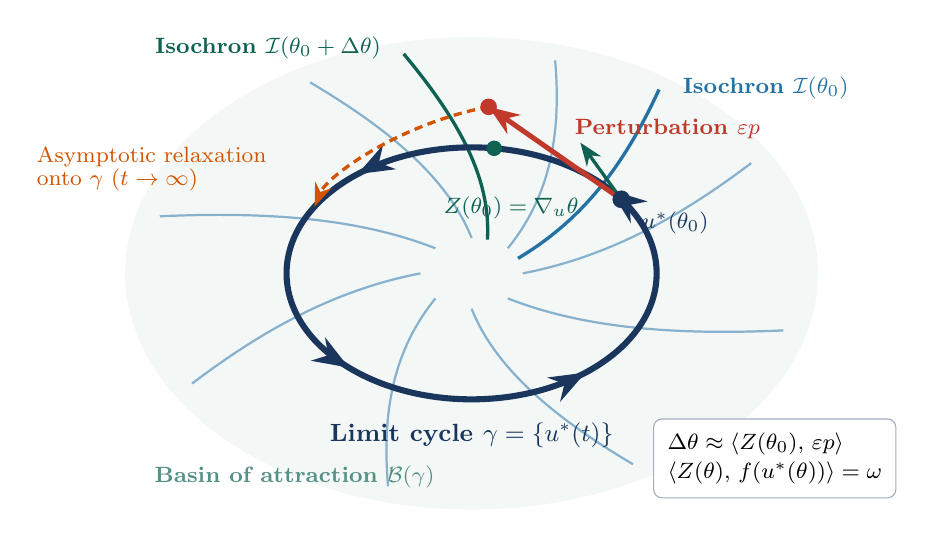
\begin{tikzpicture}[
    >=Stealth,
    font=\sffamily\small,
]

% Subtle basin backdrop
\fill[teal!5] (0,0) ellipse (4.4 and 3.0);
\node[teal!70, font=\footnotesize\bfseries, anchor=south west] at (-4.15, -2.85)
    {Basin of attraction $\mathcal{B}(\gamma)$};

% Isochrons radiating outward (curved foliations of constant asymptotic phase)
\foreach \ang/\lab in {
    0/, 45/, 90/, 135/, 180/, 225/, 270/, 315/
}{
    \draw[steelblue!55, thick]
        ({\ang}:0.65 and 0.45)
        .. controls ({\ang+10}:1.8 and 1.25) and ({\ang+22}:2.9 and 2.0) ..
        ({\ang+30}:4.1 and 2.8);
}

% Highlight two specific isochrons: I(theta_0) at 25 deg and I(theta_0 + Delta theta) at 72 deg
\draw[steelblue, very thick]
    (25:0.65 and 0.45)
    .. controls (35:1.8 and 1.25) and (47:2.9 and 2.0) ..
    (55:4.15 and 2.85);
\node[steelblue, font=\footnotesize\bfseries, anchor=west] at (53:4.25 and 2.95)
    {Isochron $\mathcal{I}(\theta_0)$};

\draw[teal, very thick]
    (72:0.65 and 0.45)
    .. controls (82:1.8 and 1.25) and (94:2.9 and 2.0) ..
    (102:4.15 and 2.85);
\node[teal, font=\footnotesize\bfseries, anchor=east] at (104:4.25 and 2.95)
    {Isochron $\mathcal{I}(\theta_0 + \Delta\theta)$};

% Limit cycle gamma (closed smooth curve with flow direction arrows)
\draw[
    navy, line width=2.2pt,
    postaction={decorate},
    decoration={
        markings,
        mark=at position 0.10 with {\arrow{Stealth}},
        mark=at position 0.37 with {\arrow{Stealth}},
        mark=at position 0.62 with {\arrow{Stealth}},
        mark=at position 0.87 with {\arrow{Stealth}},
    }
] (0,0) ellipse (2.35 and 1.60);

\node[navy, font=\bfseries\small, anchor=north] at (0, -1.78)
    {Limit cycle $\gamma = \{u^*(t)\}$};

% Base point u*(theta_0) on gamma at angle ~36 deg where highlighted I(theta_0) crosses gamma
\coordinate (u0) at (36:2.35 and 1.60);
% Perturbed point lying on I(theta_0 + Delta theta) outside gamma
\coordinate (up) at (86:3.10 and 2.12);
% Relaxed point on gamma along I(theta_0 + Delta theta)
\coordinate (u1) at (83:2.35 and 1.60);

% Perturbation vector epsilon * p
\draw[->, crimson, line width=1.8pt] (u0) -- (up)
    node[midway, above right=1pt and 3pt, crimson, font=\footnotesize\bfseries]
    {Perturbation $\varepsilon p$};

% Relaxation trajectory from perturbed point back onto limit cycle along isochron
\draw[->, amber, very thick, densely dashed]
    (up) .. controls (108:2.95 and 2.00) and (135:2.60 and 1.75) .. (148:2.35 and 1.60);
\node[amber, font=\footnotesize, align=left, anchor=east] at (142:3.15 and 2.15)
    {Asymptotic relaxation\\[-1pt]onto $\gamma$ ($t \to \infty$)};

% Gradient Z(theta_0) = grad theta normal to I(theta_0) at u0
\draw[->, teal, very thick] (u0) -- ($(u0) + (-0.52, 0.72)$);
\node[teal, font=\footnotesize\bfseries, anchor=north east] at ($(u0) + (-0.42, 0.15)$) {$Z(\theta_0) = \nabla_u \theta$};

% Points
\fill[navy] (u0) circle (3.2pt);
\node[navy, font=\footnotesize\bfseries, below right=1pt and 4pt] at (u0) {$u^*(\theta_0)$};
\fill[crimson] (up) circle (3.0pt);
\fill[teal] (u1) circle (2.8pt);

% Key formula badge in bottom-right (clear of limit cycle label)
\node[draw=navy!40, fill=white, rounded corners=3pt, align=left, font=\footnotesize, inner sep=5pt]
    at (3.85, -2.35) {%
        $\Delta\theta \approx \langle Z(\theta_0), \, \varepsilon p \rangle$\\[1pt]
        $\langle Z(\theta), \, f(u^*(\theta)) \rangle = \omega$%
    };

\end{tikzpicture}
\end{document}
